%%%%%%%%%%%%%%%%%%%%%%%%%%%%%%%%%%%%%%%%%
% NIH Grant Proposal for the Specific Aims and Research Plan Sections
% LaTeX Template
% Version 1.0 (21/10/13)
%
% This template has been downloaded from:
% http://www.LaTeXTemplates.com
%
% Original author:
% Erick Tatro (erickttr@gmail.com) with modifications by:
% Vel (vel@latextemplates.com)
%
% Adapted from:
% J. Hrabe (http://www.magalien.com/public/nih_grants_in_latex.html)
%
% License:
% CC BY-NC-SA 3.0 (http://creativecommons.org/licenses/by-nc-sa/3.0/)
%
%%%%%%%%%%%%%%%%%%%%%%%%%%%%%%%%%%%%%%%%%

%----------------------------------------------------------------------------------------
%	PACKAGES AND OTHER DOCUMENT CONFIGURATIONS
%----------------------------------------------------------------------------------------
\PassOptionsToPackage{unicode=true}{hyperref} % options for packages loaded elsewhere
\PassOptionsToPackage{hyphens}{url}
\PassOptionsToPackage{dvipsnames,svgnames*,x11names*}{xcolor}
%
%% DRS packages to load based on NIH.
\documentclass[11pt,notitlepage]{article}

% \usepackage[T1]{fontenc}
\linespread{1.15} % A little extra line spread is better for the Palatino font
\usepackage{amsfonts, amsmath, amsthm, amssymb} % For math fonts, symbols and environments
\usepackage{graphicx} % Required for including images
\usepackage{booktabs} % Top and bottom rules for table
\usepackage{wrapfig} % Allows in-line images
\usepackage{setspace}
\usepackage[labelfont=bf,font=small]{caption} % Make figure numbering in captions bold
\captionsetup{belowskip=-4pt,aboveskip=4pt}
\usepackage[top=0.5in,bottom=0.5in,left=0.5in,right=0.5in,includeheadfoot]{geometry} % Reduce the size of the margin
\usepackage[utf8]{inputenc}
\usepackage[T1]{fontenc}
\usepackage[greek,english]{babel}
% For switching to xelatex if unicode detected...
 \usepackage[no-math]{fontspec}
 \setmainfont{Helvetica}
 %\usepackage{mathspec}
 %\setmathfont(Digits,Latin)[Uppercase=Italic,Lowercase=Italic]{Helvetica}
 %\setmathfont(Greek)[Uppercase=Regular,Lowercase=Regular]{Helvetica}
 
\usepackage{fancyhdr}
\renewcommand{\headrulewidth}{0pt}
\pagestyle{fancy}
%\setlength{\headheight}{15.2pt}


 \usepackage[small,compact]{titlesec}
 \titlespacing{\title}{-2in}{0ex}{-3in}
 \titlespacing{\section}{0pt}{\parskip}{-\parskip}
 \titlespacing{\subsection}{0pt}{-\parskip}{-\parskip}
 \titlespacing{\subsubsection}{0pt}{0pt}{-\parskip}
 \titleformat{\section}%
  [hang]% <shape>
  {\normalfont\bfseries}% <format>
  {}% <label>
  {0pt}% <sep>
  {}% <before code>

\renewcommand{\thesection}{}
\renewcommand{\thesubsection}{\arabic{subsection}}

\usepackage{amssymb,amsmath}
\usepackage{ifxetex,ifluatex}
\usepackage{fixltx2e} % provides \textsubscript
\ifnum 0\ifxetex 1\fi\ifluatex 1\fi=0 % if pdftex
  \usepackage[T1]{fontenc}
  \usepackage[utf8]{inputenc}
  \usepackage{textcomp} % provides euro and other symbols
\else % if luatex or xelatex
%%  \usepackage{unicode-math}
%  \defaultfontfeatures{Ligatures=TeX,Scale=MatchLowercase}
    \setmainfont[]{Helvetica}
    \setsansfont[]{Helvetica}
%\fi
% use upquote if available, for straight quotes in verbatim environments
\IfFileExists{upquote.sty}{\usepackage{upquote}}{}
% use microtype if available
\IfFileExists{microtype.sty}{%
\usepackage[]{microtype}
\UseMicrotypeSet[protrusion]{basicmath} % disable protrusion for tt fonts
}{}
\IfFileExists{parskip.sty}{%
\usepackage{parskip}
}{% else
\setlength{\parindent}{0pt}
\setlength{\parskip}{6pt plus 2pt minus 1pt}
}
\usepackage{xcolor}
\usepackage{hyperref}
\hypersetup{
            pdftitle={Membranes, Motors, and Molecular Modeling},
            pdfauthor={David R. Slochower},
            colorlinks=true,
            linkcolor=Maroon,
            citecolor=Blue,
            urlcolor=Blue,
            breaklinks=true}
\urlstyle{same}  % don't use monospace font for urls
\usepackage{graphicx,grffile}
\makeatletter
\def\maxwidth{\ifdim\Gin@nat@width>\linewidth\linewidth\else\Gin@nat@width\fi}
\def\maxheight{\ifdim\Gin@nat@height>\textheight\textheight\else\Gin@nat@height\fi}
\makeatother
% Scale images if necessary, so that they will not overflow the page
% margins by default, and it is still possible to overwrite the defaults
% using explicit options in \includegraphics[width, height, ...]{}
\setkeys{Gin}{width=\maxwidth,height=\maxheight,keepaspectratio}
\setlength{\emergencystretch}{3em}  % prevent overfull lines
\providecommand{\tightlist}{%
  \setlength{\itemsep}{0pt}\setlength{\parskip}{0pt}}
\setcounter{secnumdepth}{5}
% Redefines (sub)paragraphs to behave more like sections
\ifx\paragraph\undefined\else
\let\oldparagraph\paragraph
\renewcommand{\paragraph}[1]{\oldparagraph{#1}\mbox{}}
\fi
\ifx\subparagraph\undefined\else
\let\oldsubparagraph\subparagraph
\renewcommand{\subparagraph}[1]{\oldsubparagraph{#1}\mbox{}}
\fi

% set default figure placement to htbp
\makeatletter
\def\fps@figure{htbp}
\makeatother


%DRS
\title{\large \vspace{-0.75in} \textbf{Membranes, Motors, and Molecular Modeling} \vspace{-1in} }
\fancypagestyle{title}{%
  \setlength{\headheight}{22pt}%
  \fancyhf{}% No header/footer
  \renewcommand{\headrulewidth}{0pt}% No header rule
  \renewcommand{\footrulewidth}{0pt}% No footer rule
  \fancyfoot[C]{\thepage}% Page number in Centre of footer
  \fancyhead[L]{David R.~Slochower}
  \fancyhead[R]{Research Plan}
}%
 \lhead{David R.~Slochower}
 \rhead{Research Plan}

% \pagestyle{empty} % Remove page numbers

\date{}

\begin{document}
% DRS
\lhead{David R.~Slochower}

\maketitle
%DRS
\thispagestyle{title}


The interface between physics and biology is an active, growing area of
science with many unanswered questions. I plan to focus on three areas
that bridge theory, modeling, and simulations. My research program will
investigate the physical principles that underlie biological and
chemical phenomena, providing new insight into the complex behavior of
cell membranes, the operation of molecular motors, and more rigorous
methods of developing force fields. I will extend my previous work in
single molecule biophysics and elucidate the driving forces that govern
the stability of sub-micron clusters featuring phosphoinositides. I seek
to use nonequilibrium kinetic modeling to develop a theory governing the
physics of artificial molecular motors and clarify design principles
that can be used to build the next generation of nanomachines. Finally,
I will help systematically overhaul force field science, changing the
way force fields are built and how they are distributed, by focusing on
transparent and rigorous optimization criteria, in an open setting.

\textcolor{blue}{\textbf{Insert university-specific paragraph here.}}

\hypertarget{use-simulations-to-understand-the-formation-of-domains-in-realistic-membrane-models}{%
\subsection{Use simulations to understand the formation of domains in
realistic membrane
models}\label{use-simulations-to-understand-the-formation-of-domains-in-realistic-membrane-models}}

{The goal of this aim is to construct quantitative models of
physiological membranes and understand the physical mechanisms that
drive the lateral segregation of lipid species.}

The primary function of a membrane is to separate what is outside from
what is inside. In simple organisms, the plasma membrane is a partition
between the complex, and sometimes delicate, molecules required for life
from the harsh environment. Mammalian plasma membranes are a rich
mixture of hundreds of types of phospholipids intermingled with other
types of lipids, sterols, and proteins. The fact that only the inner
leaflet of eukaryotic cells contains the acidic phospholipids under
physiological conditions results in a significant negative surface
charge density. Mobile counterions and proteins in the cytoplasm are
drawn to the inner leaflet of the plasma membrane, forming both specific
and non-specific interactions with membrane constituents, leading to
potentially significant alterations in membrane structure including the
formation of membrane curvature and surface patterning.

A major factor in intracellular signal transduction is the change in
phospholipid-protein binding accompanying changes in the lateral
distribution of lipids in the bilayer. Lipid redistribution can act as a
switch to turn on or off protein functions without a net change in lipid
synthesis or degradation. Negatively charged phospholipids bind
cargo-specific adaptor proteins during
endocytosis\textsuperscript{\protect\hyperlink{ref-73gnQLTS}{1}}, and
disruption in signaling pathways associated with the phosphoinositides
have been implicated in several cancers as well as neurodegenerative
disorders\textsuperscript{\protect\hyperlink{ref-8Xw2kuUO}{2}--\protect\hyperlink{ref-1DCzqvykg}{7}}.


\begin{wrapfloat}{figure}{R}{2.5in}
\centering
\includegraphics{content/images/membrane-vmd.png}
\caption{An example of a curved membrane with many different lipid
species, colored separately, representative of the systems I will
simulate.}
\label{fig:membrane-setup}
\end{wrapfloat}

Despite advances in super-resolution microscopy, such as PALM and STORM,
\emph{in vivo} characterization of membrane heterogeneity remains
challenging due to the high spatiotemporal resolution required to study
fluctuating nanoscale assemblies of lipids and proteins in living cells
and the need to chemically modify the lipids or bind them to ligands in
order to visualize them or detect their motions and conformations by
spectroscopy. However, a variety of indirect experimental techniques,
often using fluorescently labeled lipid analogs, have characterized the
existence of sub-micron sized domains in living cells and plasma
membrane
extracts\textsuperscript{\protect\hyperlink{ref-GGtK2c0N}{8}--\protect\hyperlink{ref-aiu6Tmil}{12}}.
Even in the absence of proteins or chemical modifications, \emph{in
vitro} assays in the Janmey group have demonstrated clusters of
negatively charged phospholipids of on the order of 50 nm after the
addition of as little as 1 μM
Ca\textsuperscript{2+}\textsuperscript{\protect\hyperlink{ref-LhOwGz4k}{13}}.

My approach is to understand what conditions promote cluster formation
and how the behavior of lipids in clusters differs from bulk. I will
initially focus on delineating the nucleation of cation-induced clusters
of anionic phospholipids. This work will involve extending the methods I
developed to investigate single molecule QM/MM and all-atom nanoscale
simulations. In those simulations, I found that Ca\textsuperscript{2+}
can act as ``molecular glue,'' forming aggregates of three lipids that
remain together for at least 100 ns, much longer than other ion-lipid
bond lifetimes. Extending beyond the all-atom simulations, I will use
the \href{https://github.com/biophyscode}{methods} we created to
construct and equilibrate multi-component membrane systems to build
models containing rich mixtures of phospholipids (Figure
\ref{fig:membrane-setup}), going past typical two or three-component
systems that are frequently used.

The finite and well-defined size of the domains suggests there is a
balance between the mutual electrostatic and steric repulsion of
negatively charged lipids and attraction mediated by counterions. I will
monitor the extent of phase separation and demixing in simulations
containing combinations of physiological divalent and monovalent ions
with varying fractions of charged and uncharged lipids. The calculated
diffusion coefficient inside the clusters can be compared with values
obtained using fluorescence correlation spectroscopy (FCS) and spot
variant FCS\textsuperscript{\protect\hyperlink{ref-oBaB5Z87}{10}}.
Simple, physical models based primarily on
electrostatics\textsuperscript{\protect\hyperlink{ref-10CqL9t0a}{14}}
predict continual growth of clusters in the presence of excess
counterions, yet \emph{in vivo} clusters plateau at a stable size.
Taking advantage of multiscale techniques, including all-atom and
coarse-grained simulations using GPU-accelerated molecular dynamics, I
will be able to study the growth and merging of clusters on the
biologically-relevant microsecond to millisecond timescale. The size and
shape of the simulated clusters will be contrasted with those seen with
AFM imaging and electron
microscopy\textsuperscript{\protect\hyperlink{ref-LhOwGz4k}{13}}.

Experiments pulling thin membrane tethers have shown that
phase-separated phospholipid domains form precisely at the junction of
highly curved
regions\textsuperscript{\protect\hyperlink{ref-XIltXoGI}{15}}, implying
a relationship between membrane morphology and lipid sorting. The
bending modulus and mean curvature of simulated clusters will be
compared with data from pipette aspiration of membrane
tubules\textsuperscript{\protect\hyperlink{ref-oBaB5Z87}{10},\protect\hyperlink{ref-aiu6Tmil}{12},\protect\hyperlink{ref-XIltXoGI}{15}},
and the order parameter of lipids inside the cluster can be contrasted
with complementary non-fluorescent methods, such as EPR, NMR, and
neutron scattering.


\begin{wrapfloat}{figure}{L}{2in}
\centering
\includegraphics{content/images/stereospecific.png}
\caption{An illustration of stereospecific recognition of phospholipids
by proteins.}
\label{fig:stereospecific}
\end{wrapfloat}

Finally, I will study whether being in a cluster alters the ability of
certain lipids to perform their biological roles. Many of the lipids
implicated in cluster formation, such as
PtdIns(4,5)\emph{P}\textsubscript{2}, have been shown to bind hundreds
of proteins\textsuperscript{\protect\hyperlink{ref-uyKE7bWV}{16}}, and
several integral membrane proteins have been shown to partition into
lipid raft-like
domains\textsuperscript{\protect\hyperlink{ref-2TfZ4zWV}{17}}. In some
cases, PtdIns(4,5)\emph{P}\textsubscript{2} binds protein pockets in a
highly stereospecific manner (i.e., PtdIns(4,5)\emph{P}\textsubscript{2}
may bind tightly but the closely related isomers
PtdIns(3,5)\emph{P}\textsubscript{2} and
PtdIns(3,5)\emph{P}\textsubscript{2} may not bind at all) requiring a
fully extended and accessible head group (Figure
\ref{fig:stereospecific}). In order to evaluate the biological
consequences of clustering, I will run simulations containing proteins
that bind through either non-specific, electrostatic attraction (e.g.,
N-WASP and gelsolin) or through tight coordination (e.g., the PH domain
of PLCδ). Whether these proteins bind ``free'' lipid molecules as well
as they bind clustered ones will be evaluated by using steered molecular
dynamics.

I expect the outcome of studying domain formation to be especially
helpful for building better models of plasma membranes that reflect the
complex cellular environment. I anticipate these results could provide
quantitative insights for pore-formation in cell membranes by toxins and
cationic surfactants, the activation of integral ion channels and GPCRs
by PtdIns(4,5)\emph{P}\textsubscript{2}, and the dynamics of membrane
fusion, fission and other buckling geometries.

\hypertarget{develop-a-physical-theory-of-molecular-motors}{%
\subsection{Develop a physical theory of molecular
motors}\label{develop-a-physical-theory-of-molecular-motors}}

{The proposed research will investigate the mechanical properties of
existing synthetic molecular motors and suggest new design routes for
future nanomachines.}


\begin{wrapfloat}{figure}{L}{2in}
\centering
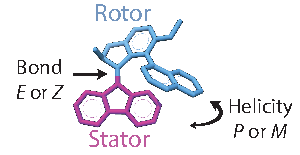
\includegraphics{content/images/motor.png}
\caption{The two degrees of freedom in a synthetic molecular motor.}
\label{fig:motor-diagram}
\end{wrapfloat}

The ability of light-driven molecular motors to switch between two or
more states makes them suitable for new forms of optical data
storage\textsuperscript{\protect\hyperlink{ref-18PGyWtWV}{18}}, as
``wheels'' on nano-scale
cars\textsuperscript{\protect\hyperlink{ref-OAnfwOYX}{19}},
trains\textsuperscript{\protect\hyperlink{ref-10MPrT2Vf}{20}},
worms\textsuperscript{\protect\hyperlink{ref-Tels98bO}{21}}, and
walkers\textsuperscript{\protect\hyperlink{ref-SfUEsk0e}{22}}, or in new
forms of responsive
materials\textsuperscript{\protect\hyperlink{ref-jCuccJLJ}{23}}. While
it is clear that artificial motors, when aligned appropriately so their
individual effects are magnified, can produce macroscopic effects, it is
not known how much force an individual molecular motor can generate. I
plan to develop a statistical mechanical theory that characterizes the
out-of-equilibrium conformational cycling of rotary molecular motors. I
will apply the nonequilibrium model I developed to quantify directional
motion in biological motors to these artificial motors, initially
focusing on the ``second generation'' class of motors from Ben Feringa
and colleagues\textsuperscript{\protect\hyperlink{ref-FwAqK1Dt}{24}}.
These motors belong to a class of molecules called overcrowded alkenes,
with two stable enantiomers, and adopt a helical shape due to steric
strain around the central double bond. Upon irradiation with light and
the application of heat, the two sets of conjugated rings rotate
relative to each other, with the central bond acting as an axle, and for
simplicity, one set of rings is designated the ``stator'' while the
other set is called the ``rotor.'' The directional motion of these
molecules can be analyzed in terms of two degrees of freedom: \(E\) to
\(Z\) for the isomerization of the double bond (analogous to \emph{cis}
and \emph{trans}) and \(P\) and \(M\) for the overall twist or helicity
of the molecule (Figure \ref{fig:motor-diagram}).

To start, I will study the four ground states that comprise the
360\(^\circ\) cycle of the motor depicted in Figure \ref{fig:motors}.
The ground state structures can be mapped onto discretized potential
energy surfaces (PES) for each isomerization state, that will be
determined evaluating the ground state energy of the motor as a function
of the central dihedral angle. A Markov matrix encodes the rates of
moving between and along bins on each PES, and the eigenvectors of this
matrix characterize the steady state probability flux that quantifies
the extent of directional motion. From this, I can determine the maximum
speed and the maximum power that can be produced by individual motors.

\begin{figure}
\centering
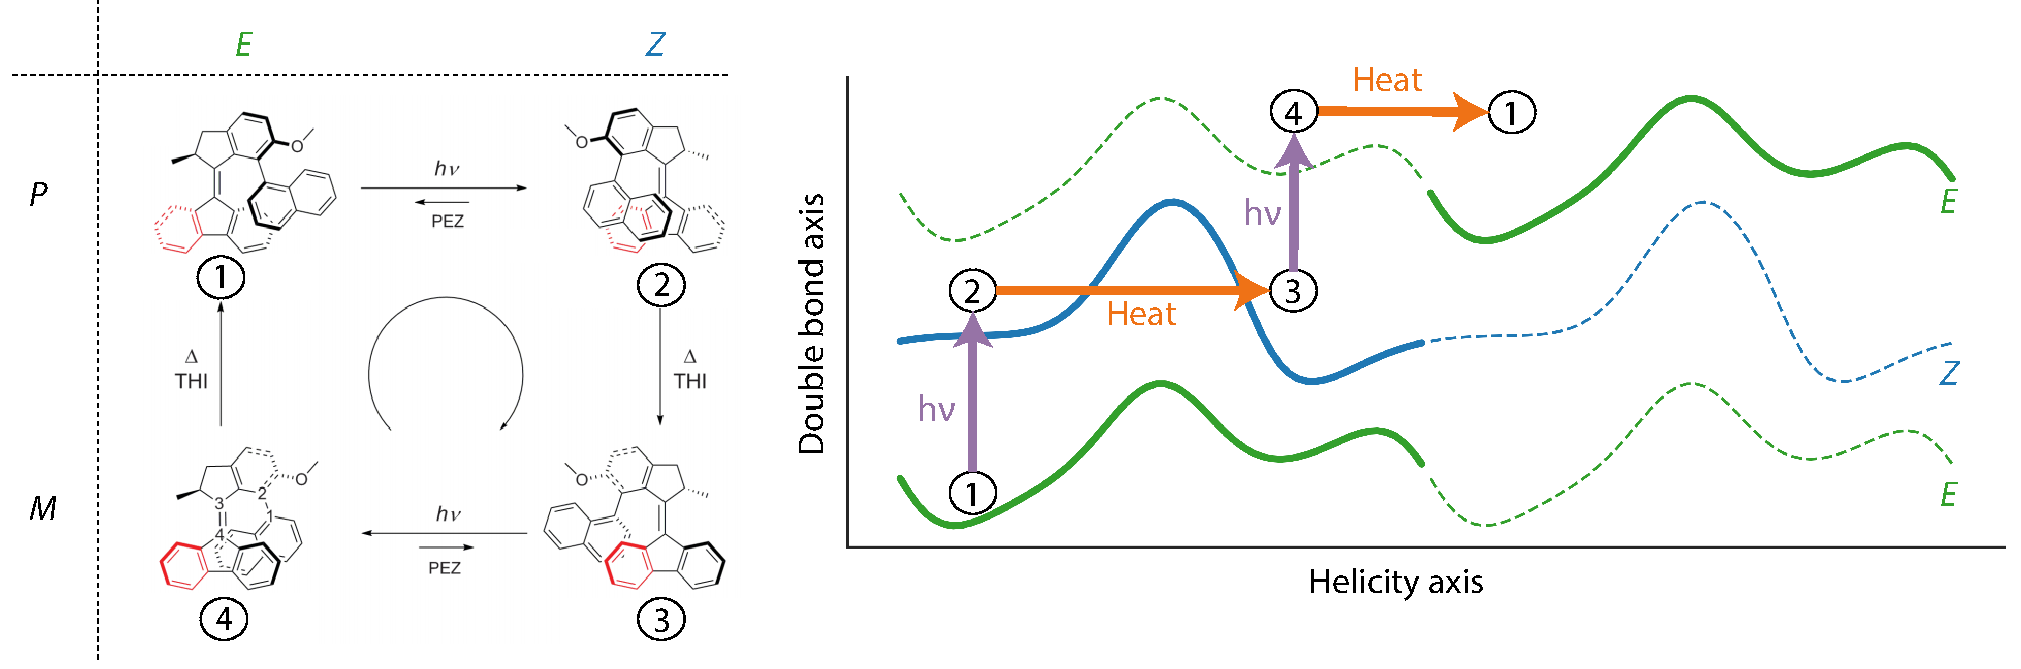
\includegraphics[width=1\textwidth,height=\textheight]{content/images/offset-barriers.png}
\caption{On the left, the four ground state conformations of a second
generation motor, adapted from Štacko et
al\textsuperscript{\protect\hyperlink{ref-mKSNFvW7}{25}}. On the right,
the same four states placed on free energy profiles. The energy profiles
are periodic, with two cycles shown for either isomerization state. A
clone of the lower \(E\) energy surface is shown above, for clarity, to
demonstrate the progression from state 4 to state 1 requires
energy.\label{fig:motors}}
\end{figure}

Over the past decade, there have been many designs for rotary motors
(reviewed by Kassem et
al.\textsuperscript{\protect\hyperlink{ref-1H5r7SBir}{26}}), and it has
become clear that the chemical constituents on both the rotor and the
stator affect motor
operation\textsuperscript{\protect\hyperlink{ref-MVPWALSk}{27}}.
Reducing the bulkiness of the rotor can speed up the overall rotation
rate of the motor, but can also lead to the loss of
directionality\textsuperscript{\protect\hyperlink{ref-1F5wsgY82}{28}}.
It is also possible to alter the quantum yield of the photochemical step
by adding electron withdrawing or electron donating groups, polarizing
the molecule and lengthening the central double
bond\textsuperscript{\protect\hyperlink{ref-Ewc7FKL8}{29},\protect\hyperlink{ref-122TltEto}{30}}.
However, to date there is no underlying theory that can be leveraged to
aid the creation of new motors.

As demonstrated by Richard Feynman in a lecture on Brownian ratchets,
the challenge of designing molecular motors is not how to create
movement, but how to control the directionality of the omnipresent --
and random -- motion on the molecular
scale\textsuperscript{\protect\hyperlink{ref-10FsKpWBI}{31}}. This has
been referred to as the ``gating'' of stochastic
motion\textsuperscript{\protect\hyperlink{ref-qhUBHBOM}{32}}. In my
previous work\textsuperscript{\protect\hyperlink{ref-1BfYw0gk2}{33}}, I
showed that the gating can arise purely from the complementary shape of
two PES, whereby an unpassable barrier on one surface can be
circumnavigated by motion on the other surface (see Figure S6, in
particular.)

By systematically studying how the addition of chemical moieties affects
the \(E\) and \(Z\) PES of the motors, the relationship between the
chemical makeup of the rotor and stator and the strength of directional
motion will become clear. The understanding gained from this analysis
can be used to suggest new avenues in chemical space to create rotors
geared for a particular purpose. For example, in some instances it may
be desirable to have motors that rotate slowly but provide a tremendous
amount of torque (e.g., for using nanoscale motors to transport
macroscopic objects) while in other circumstances, it may be more
beneficial to have motors that rotate as quickly as possible (e.g., for
using motors to rapidly switch the surface properties of a particular
material). The results of this research will provide a fundamental
understanding of the principles underlying motor operation and open up
rational design for molecular rotors, pumps, transporters, and other
nanorobotics.

\hypertarget{building-better-force-fields-for-drug-discovery-using-open-data-and-automated-optimization}{%
\subsection{Building better force fields for drug discovery using open
data and automated
optimization}\label{building-better-force-fields-for-drug-discovery-using-open-data-and-automated-optimization}}

{The proposed research in this aim will change the way force fields are
built and the way they are optimized, to improve their accuracy on
biomedical problems.}

Designing ligands that bind their target with high affinity and
specificity is the principal objective of small-molecule drug discovery,
yet hit-to-lead and lead-optimization can take upwards of three years
owing to the fact it is often necessary to synthesize hundreds or
thousands of new compounds. In short, drug discovery is very expensive
and often fails. In recent years, the pharmaceutical industry has begun
to use absolute and relative binding free energy calculations to help
narrow the number of compounds that must be
synthesized\textsuperscript{\protect\hyperlink{ref-1FiDpP1LR}{34},\protect\hyperlink{ref-1BwXH3GFO}{35}}.
In particular, the advent of computational calorimetry has enabled
quantitative and high-precision comparisons of binding free energies,
enthalpies, and entropies (by subtraction) with experimental values
determined by isothermal titration calorimetry or
NMR\textsuperscript{\protect\hyperlink{ref-1935a9V0d}{36}}. The root
mean squared error associated with such calculations is several
kcal/mol\textsuperscript{\protect\hyperlink{ref-LWd10vQy}{37}}, and even
a modest improvement of the prediction accuracy by 1 kcal/mol would lead
to a substantial decrease in the number of compounds that must be
manually screened\textsuperscript{\protect\hyperlink{ref-fC0t6Cy1}{38}}.
Although it has been suggested by some that changes in the force field
functional form are required, it is clear that there is ample room to
improve the accuracy of existing parameters through careful
analysis\textsuperscript{\protect\hyperlink{ref-LOjcxYqt}{39}}. The
first goal of this aim is to create better tools to guide early-stage
drug discovery by reducing the number of compounds that must be
synthesized to find a promising hit that can be carried over into
clinical trials.


\begin{wrapfloat}{figure}{L}{3in}
\centering
\includegraphics{content/images/APR-annotated.png}
\caption{An example host-guest system, \(\alpha\)-cyclodextrin with
cyclooctanol (unbound) showing the pulling coordinate along the \(z\)
axis.}
\label{fig:apr}
\end{wrapfloat}

While it would be ideal to predict the binding affinity of candidate
ligands to proteins, the long sampling required to reach convergence on
such systems renders them unsuitable for rapid testing. Host-guest
systems are noncovalent complexes between a cavity-like host molecule
and a small molecule guest. These systems retain many of the same,
strong functional group interactions of protein-ligand systems while
being computationally tractable. In the attach-pull-release (APR)
method, the reversible work of transferring the guest from the binding
site to solution, via a physical pathway, is computed using a series of
umbrella sampling windows (Figure \ref{fig:apr}). In the ``attach''
phase, restraints are connected to the guest (and optionally, to the
host for better conformational sampling) through a parameter
\(\lambda \in [0, 1]\) that controls the strength of the restraints.
During the ``pull'' phase, the equilibrium length of a distance
restraint joining the guest and host is increased until the guest is no
longer interacting with the host molecule. The ``release'' phase
reverses the work of attaching the restraints and also corrects the
concentration of the guest molecule to standard state. Simulating each
window and integrating over the partial derivative of the restraint
energy with respect to the restraint target, we can generate a potential
of mean force along the pulling coordinate that is used to compute the
binding free energy at standard state, \(\Delta G^\circ\).

APR has consistently been ranked among the most accurate methods for
predicting binding thermodynamics in blind
challenges\textsuperscript{\protect\hyperlink{ref-BGsUYQln}{40},\protect\hyperlink{ref-GA1AFcUw}{41}}.
I will independently continue the development of APR, and its Python
interface that I developed -- called pAPRika -- by transforming it into
a generalized tool that is capable of computing free energies along any
physical pathway, using either AMBER or OpenMM as simulation packages.
The core functionality of pAPRika is already being used by research
groups across the country and in at least one group in China. Extending
pAPRika would allow the same rigorous thermodynamic framework to be used
in applications such as protein-protein interactions, dimerization of
small molecules, or nucleotide flipping. As part of the development, I
will also investigate the accuracy of non-pathway, end-point methods,
such as the direct calculation of interaction
entropy\textsuperscript{\protect\hyperlink{ref-gRfhPG7N}{42}}.

Most established small molecule force fields (e.g., the general AMBER
force field, GAFF) have been tuned using pure liquid state data, such as
the average density, enthalpy of vaporization, or the self-diffusion
coefficient. Over the past decade, it has become clear that reproducing
those properties well does not guarantee binding thermodynamics at a
level acceptable for guiding experiments. The open force field group
(OpenFF) aims to develop new, collaborative force fields using open
access methods, open source software, and high-quality open data sets.
One central difference with the OpenFF group is the use of direct
chemical perception to apply force field parameters based on a molecular
graph instead of atom
types\textsuperscript{\protect\hyperlink{ref-HlBr7NrU}{43}}, and the
desire to avoid over-fitting parameters by making Monte Carlo moves in
parameter space to find the fewest number of parameters required to
describe a set of
chemistries\textsuperscript{\protect\hyperlink{ref-13lTSBgHy}{44}}. The
first prototype force field from this effort was release in June 2018,
called SMIRNOFF99Frosst v0.1, based on a predecessor of GAFF.
SMIRNOFF99Frosst is able to perform as well as GAFF, and in some cases,
alleviate conformational problems caused by GAFF's atom types, in only
335 parameter lines compared to the 6794 lines in GAFF version 2.1.
Beyond this initial release, multiple generations of SMIRNOFF-based
force fields are planned, incorporating new forms of Lennard-Jones
interactions, the addition of atom polarizabilities, and Bayesian
estimates to quantify systematic errors in the force field.


\begin{wrapfloat}{figure}{R}{3in}
\centering
\includegraphics{content/images/SMIRNOFF-vs-GAFF-deltaG.png}
\caption{A comparison of binding free energies between SMIRNOFF99Frosst
and GAFF v1.7 for a series of cyclodextrin hosts and guests (unpublished
results). Points are colored according to guest functional group.}
\label{fig:smirnoff}
\end{wrapfloat}

As a member of the OpenFF consortium, I am responsible for benchmarking
new iterations of SMIRNOFF-family force fields using host-guest
thermodynamics computed by pAPRika. Figure \ref{fig:smirnoff} shows the
very first comparison of SMIRNOFF99Frosst v0.1 and GAFF v1.7 on
host-guest systems. GAFF v1.7 is known to overestimate binding
affinities by \textgreater{}1
kcal/mol\textsuperscript{\protect\hyperlink{ref-HVgz5rZq}{45}}, and it
appears that SMIRNOFF99Frosst reduces this tendency. To begin, I will
use the ``\href{https://escholarship.org/uc/item/9p37m6bq}{benchmark
set}'' of Mobley et
al.\textsuperscript{\protect\hyperlink{ref-12BD3oHp4}{46}}. There,
experimental data are available for rigid curcurbituril and highly
flexible cyclodextrin hosts with a variety of drug-like guest molecules.
When available, I plan to incorporate the binding data resulting from
selective derivatization of cyclodextrins designed to evaluate specific
functional group
interactions\textsuperscript{\protect\hyperlink{ref-13gqBX78S}{47}}.
Enthalpies are poorly correlated with free energies, and thus, they
represent a nearly independent set of data to compare. pAPRika makes it
easy to match the simulations to the experimental conditions, including
host and guest concentration, stoichiometry, ion concentration, and
buffer conditions.

To integrate the pAPRika calculations with the OpenFF group, I will
leverage the ForceBalance framework. ForceBalance is a tool, written by
Dr.~Lee-Ping Wang, that uses thermodynamic fluctuation formulas and
reference data (e.g., \emph{ab initio} quantum mechanical calculations
and experimentally known molecular or bulk properties) to optimize an
objective function, such as the sum of squared differences between the
calculated and reference values. ForceBalance has already been used to
optimize water
models\textsuperscript{\protect\hyperlink{ref-50lAQZra}{48}} and protein
force fields\textsuperscript{\protect\hyperlink{ref-1E3wArY0j}{49}}. As
a member of the OpenFF consortium, Dr.~Wang has begun to add support for
the SMIRNOFF force field format. I will extend my collaboration with
Dr.~Wang to include pAPRika in the optimization loop of ForceBalance. I
have experience working with the analytic derivatives of the binding
free energy with respect to Lennard-Jones
parameters\textsuperscript{\protect\hyperlink{ref-xRauI5mb}{50}}, and
using these derivatives to tune parameters was recently used by a
colleague to optimize the TIP3P water model for binding calculations by
post-processing existing MD trajectories for small parameter
perturbation\textsuperscript{\protect\hyperlink{ref-NeqIQDLp}{51}}.

Together, these methodological improvements will help create a
transparent and robust set of metrics to evaluate the performance of
candidate force fields on an equal footing. By incorporating host-guest
binding data, the degeneracy in parameter space will be broken, avoiding
force fields that agree excellently with experiment for liquid
properties and yet agree poorly on binding. I believe the ideas in this
aim could be turned into an NIH proposal by demonstrating the need to
systematically evaluate force field accuracy for protein-ligand binding,
perhaps the most important application of this work for human health.

\pagebreak
\setlength{\parskip}{0.1mm}

\hypertarget{references}{%
\section*{References}\label{references}}
\addcontentsline{toc}{section}{References}

\setstretch{1}

\hypertarget{refs}{}
\leavevmode\hypertarget{ref-73gnQLTS}{}%
(1) Ramanan, V.; Agrawal, N. J.; Liu, J.; Engles, S.; Toy, R.;
Radhakrishnan, R. Systems Biology and Physical Biology of
Clathrin-Mediated Endocytosis. \emph{Integr. Biol.} \textbf{2011},
\emph{3} (8), 803.

\leavevmode\hypertarget{ref-8Xw2kuUO}{}%
(2) Faiderbe, S.; Chagnaud, J.-L.; Geffard, M. Anti-Phosphoinositide
Auto-Antibodies in Sera of Cancer Patients: Isotypic and Immunochemical
Characterization. \emph{Cancer Letters} \textbf{1992}, \emph{66} (1),
35--41.

\leavevmode\hypertarget{ref-12CAxA8dE}{}%
(3) Lin, W.; Leung, L. W.; Bae, Y. S.; Bittman, R.; Arthur, G. Effects
of a Water-Soluble Antitumor Ether Phosphonoinositide, d-Myo-Inositol
4-(Hexadecyloxy)-3(S)-Methoxybutanephosphonate (C4-Pi), on Inositol
Lipid Metabolism in Breast Epithelial Cancer Cell Lines.
\emph{Biochemical Pharmacology} \textbf{1999}, \emph{57} (10),
1153--1158.

\leavevmode\hypertarget{ref-l2gqdgv}{}%
(4) Katso, R.; Okkenhaug, K.; Ahmadi, K.; White, S.; Timms, J.;
Waterfield, M. D. Cellular Function of Phosphoinositide 3-Kinases:
Implications for Development, Immunity, Homeostasis, and Cancer.
\emph{Annu. Rev. Cell Dev. Biol.} \textbf{2001}, \emph{17} (1),
615--675.

\leavevmode\hypertarget{ref-izLqFTEH}{}%
(5) Engelman, J. A. The Role of Phosphoinositide 3-Kinase Pathway
Inhibitors in the Treatment of Lung Cancer. \emph{Clinical Cancer
Research} \textbf{2007}, \emph{13} (15), 4637s--4640s.

\leavevmode\hypertarget{ref-1HRoQaadQ}{}%
(6) Miled, N.; Yan, Y.; Hon, W.-C.; Perisic, O.; Zvelebil, M.; Inbar,
Y.; Schneidman-Duhovny, D.; Wolfson, H. J.; Backer, J. M.; Williams, R.
L. Mechanism of Two Classes of Cancer Mutations in the Phosphoinositide
3-Kinase Catalytic Subunit. \emph{Science} \textbf{2007}, \emph{317}
(5835), 239--242.

\leavevmode\hypertarget{ref-1DCzqvykg}{}%
(7) Bunney, T. D.; Katan, M. Phosphoinositide Signalling in Cancer:
Beyond PI3K and PTEN. \emph{Nat Rev Cancer} \textbf{2010}, \emph{10}
(5), 342--352.

\leavevmode\hypertarget{ref-GGtK2c0N}{}%
(8) Gidwani, A.; Holowka, D.; Baird, B. Fluorescence Anisotropy
Measurements of Lipid Order in Plasma Membranes and Lipid Rafts from
RBL-2H3 Mast Cells†. \emph{Biochemistry} \textbf{2001}, \emph{40} (41),
12422--12429.

\leavevmode\hypertarget{ref-1Eg1Hzju1}{}%
(9) Swamy, M. J.; Ciani, L.; Ge, M.; Smith, A. K.; Holowka, D.; Baird,
B.; Freed, J. H. Coexisting Domains in the Plasma Membranes of Live
Cells Characterized by Spin-Label ESR Spectroscopy. \emph{Biophysical
Journal} \textbf{2006}, \emph{90} (12), 4452--4465.

\leavevmode\hypertarget{ref-oBaB5Z87}{}%
(10) Levental, I.; Byfield, F.; Chowdhury, P.; Gai, F.; Baumgart, T.;
Janmey, P. Cholesterol-Dependent Phase Separation in Cell-Derived Giant
Plasma-Membrane Vesicles. \emph{Biochem. J.} \textbf{2009}, \emph{424}
(2), 163--167.

\leavevmode\hypertarget{ref-BzP79Vj9}{}%
(11) Sengupta, P.; Holowka, D.; Baird, B. Fluorescence Resonance Energy
Transfer Between Lipid Probes Detects Nanoscopic Heterogeneity in the
Plasma Membrane of Live Cells. \emph{Biophysical Journal} \textbf{2007},
\emph{92} (10), 3564--3574.

\leavevmode\hypertarget{ref-aiu6Tmil}{}%
(12) Baumgart, T.; Hammond, A. T.; Sengupta, P.; Hess, S. T.; Holowka,
D. A.; Baird, B. A.; Webb, W. W. Large-Scale Fluid/Fluid Phase
Separation of Proteins and Lipids in Giant Plasma Membrane Vesicles.
\emph{Proceedings of the National Academy of Sciences} \textbf{2007},
\emph{104} (9), 3165--3170.

\leavevmode\hypertarget{ref-LhOwGz4k}{}%
(13) Wang, Y.-H.; Collins, A.; Guo, L.; Smith-Dupont, K. B.; Gai, F.;
Svitkina, T.; Janmey, P. A. Divalent Cation-Induced Cluster Formation by
Polyphosphoinositides in Model Membranes. \emph{J. Am. Chem. Soc.}
\textbf{2012}, \emph{134} (7), 3387--3395.

\leavevmode\hypertarget{ref-10CqL9t0a}{}%
(14) Ellenbroek, W.; Wang, Y.-H.; Christian, D.; Discher, D.; Janmey,
P.; Liu, A. Divalent Cation-Dependent Formation of Electrostatic PIP2
Clusters in Lipid Monolayers. \emph{Biophysical Journal} \textbf{2011},
\emph{101} (9), 2178--2184.

\leavevmode\hypertarget{ref-XIltXoGI}{}%
(15) Heinrich, M.; Tian, A.; Esposito, C.; Baumgart, T. Dynamic Sorting
of Lipids and Proteins in Membrane Tubes with a Moving Phase Boundary.
\emph{Proceedings of the National Academy of Sciences} \textbf{2010},
\emph{107} (16), 7208--7213.

\leavevmode\hypertarget{ref-uyKE7bWV}{}%
(16) Lemmon, M. A. Membrane Recognition by Phospholipid-Binding Domains.
\emph{Nat Rev Mol Cell Biol} \textbf{2008}, \emph{9} (2), 99--111.

\leavevmode\hypertarget{ref-2TfZ4zWV}{}%
(17) Raghunathan, K.; Kenworthy, A. K. Dynamic Pattern Generation in
Cell Membranes: Current Insights into Membrane Organization.
\emph{Biochimica et Biophysica Acta (BBA) - Biomembranes} \textbf{2018},
\emph{1860} (10), 2018--2031.

\leavevmode\hypertarget{ref-18PGyWtWV}{}%
(18) Feringa, B.; Koumura, N.; van Delden, R.; ter Wiel, M. Light-Driven
Molecular Switches and Motors. \emph{Appl Phys A} \textbf{2002},
\emph{75} (2), 301--308.

\leavevmode\hypertarget{ref-OAnfwOYX}{}%
(19) Kudernac, T.; Ruangsupapichat, N.; Parschau, M.; Maciá, B.;
Katsonis, N.; Harutyunyan, S. R.; Ernst, K.-H.; Feringa, B. L.
Electrically Driven Directional Motion of a Four-Wheeled Molecule on a
Metal Surface. \emph{Nature} \textbf{2011}, \emph{479} (7372), 208--211.

\leavevmode\hypertarget{ref-10MPrT2Vf}{}%
(20) Sasaki, T.; Guerrero, J. M.; Leonard, A. D.; Tour, J. M. Nanotrains
and Self-Assembled Two-Dimensional Arrays Built from Carboranes Linked
by Hydrogen Bonding of Dipyridones. \emph{Nano Res.} \textbf{2008},
\emph{1} (5), 412--419.

\leavevmode\hypertarget{ref-Tels98bO}{}%
(21) Sasaki, T.; Tour, J. M. Synthesis of a New Photoactive
Nanovehicle:~ A Nanoworm. \emph{Org. Lett.} \textbf{2008}, \emph{10}
(5), 897--900.

\leavevmode\hypertarget{ref-SfUEsk0e}{}%
(22) von Delius, M.; Leigh, D. A. Walking Molecules. \emph{Chem. Soc.
Rev.} \textbf{2011}, \emph{40} (7), 3656.

\leavevmode\hypertarget{ref-jCuccJLJ}{}%
(23) Lucas, L. N.; van Esch, J.; Feringa, B. L.; Kellogg, R. M.
Photocontrolled Self-Assembly of Molecular Switches. \emph{Chem.
Commun.} \textbf{2001}, No. 8, 759--760.

\leavevmode\hypertarget{ref-FwAqK1Dt}{}%
(24) Klok, M.; Walko, M.; Geertsema, E.; Ruangsupapichat, N.;
Kistemaker, J.; Meetsma, A.; Feringa, B. New Mechanistic Insight in the
Thermal Helix Inversion of Second-Generation Molecular Motors.
\emph{Chem. Eur. J.} \textbf{2008}, \emph{14} (35), 11183--11193.

\leavevmode\hypertarget{ref-mKSNFvW7}{}%
(25) Štacko, P.; Kistemaker, J. C. M.; van Leeuwen, T.; Chang, M.-C.;
Otten, E.; Feringa, B. L. Locked Synchronous Rotor Motion in a Molecular
Motor. \emph{Science} \textbf{2017}, \emph{356} (6341), 964--968.

\leavevmode\hypertarget{ref-1H5r7SBir}{}%
(26) Kassem, S.; van Leeuwen, T.; Lubbe, A. S.; Wilson, M. R.; Feringa,
B. L.; Leigh, D. A. Artificial Molecular Motors. \emph{Chem. Soc. Rev.}
\textbf{2017}, \emph{46} (9), 2592--2621.

\leavevmode\hypertarget{ref-MVPWALSk}{}%
(27) Bauer, J.; Hou, L.; Kistemaker, J. C. M.; Feringa, B. L. Tuning the
Rotation Rate of Light-Driven Molecular Motors. \emph{J. Org. Chem.}
\textbf{2014}, \emph{79} (10), 4446--4455.

\leavevmode\hypertarget{ref-1F5wsgY82}{}%
(28) ter Wiel, M. K. J.; van Delden, R. A.; Meetsma, A.; Feringa, B. L.
Increased Speed of Rotation for the Smallest Light-Driven Molecular
Motor. \emph{J. Am. Chem. Soc.} \textbf{2003}, \emph{125} (49),
15076--15086.

\leavevmode\hypertarget{ref-Ewc7FKL8}{}%
(29) Filatov, M.; Olivucci, M. Designing Conical Intersections for
Light-Driven Single Molecule Rotary Motors: From Precessional to Axial
Motion. \emph{J. Org. Chem.} \textbf{2014}, \emph{79} (8), 3587--3600.

\leavevmode\hypertarget{ref-122TltEto}{}%
(30) Nikiforov, A.; Gamez, J. A.; Thiel, W.; Filatov, M. Computational
Design of a Family of Light-Driven Rotary Molecular Motors with Improved
Quantum Efficiency. \emph{J. Phys. Chem. Lett.} \textbf{2015}, \emph{7}
(1), 105--110.

\leavevmode\hypertarget{ref-10FsKpWBI}{}%
(31) Browne, W. R.; Feringa, B. L. Making Molecular Machines Work.
\emph{Nature Nanotech} \textbf{2006}, \emph{1} (1), 25--35.

\leavevmode\hypertarget{ref-qhUBHBOM}{}%
(32) Astumian, R. D. Stochastic Pumping of Non-Equilibrium
Steady-States: How Molecules Adapt to a Fluctuating Environment.
\emph{Chem. Commun.} \textbf{2018}, \emph{54} (5), 427--444.

\leavevmode\hypertarget{ref-1BfYw0gk2}{}%
(33) Slochower, D. R.; Gilson, M. K. Motor-Like Properties of Nonmotor
Enzymes. \emph{Biophysical Journal} \textbf{2018}, \emph{114} (9),
2174--2179.

\leavevmode\hypertarget{ref-1FiDpP1LR}{}%
(34) van Vlijmen, H.; Desjarlais, R. L.; Mirzadegan, T. Computational
Chemistry at Janssen. \emph{J Comput Aided Mol Des} \textbf{2016},
\emph{31} (3), 267--273.

\leavevmode\hypertarget{ref-1BwXH3GFO}{}%
(35) Christ, C. D.; Fox, T. Accuracy Assessment and Automation of Free
Energy Calculations for Drug Design. \emph{J. Chem. Inf. Model.}
\textbf{2013}, \emph{54} (1), 108--120.

\leavevmode\hypertarget{ref-1935a9V0d}{}%
(36) Henriksen, N. M.; Fenley, A. T.; Gilson, M. K. Computational
Calorimetry: High-Precision Calculation of Host--Guest Binding
Thermodynamics. \emph{J. Chem. Theory Comput.} \textbf{2015}, \emph{11}
(9), 4377--4394.

\leavevmode\hypertarget{ref-LWd10vQy}{}%
(37) Gaieb, Z.; Liu, S.; Gathiaka, S.; Chiu, M.; Yang, H.; Shao, C.;
Feher, V. A.; Walters, W. P.; Kuhn, B.; Rudolph, M. G.; et al. D3R Grand
Challenge 2: Blind Prediction of Protein--Ligand Poses, Affinity
Rankings, and Relative Binding Free Energies. \emph{J Comput Aided Mol
Des} \textbf{2017}, \emph{32} (1), 1--20.

\leavevmode\hypertarget{ref-fC0t6Cy1}{}%
(38) Shirts, M. R.; Mobley, D. L.; Brown, S. P. Free-Energy Calculations
in Structure-Based Drug Design. In \emph{Drug Design: Structure- and
Ligand-Based Approaches}; Merz Jr., K. M., Ringe, D., Reynolds, C. H.,
Series Eds.; Cambridge University Press, 2010.

\leavevmode\hypertarget{ref-LOjcxYqt}{}%
(39) Fennell, C. J.; Wymer, K. L.; Mobley, D. L. A Fixed-Charge Model
for Alcohol Polarization in the Condensed Phase, and Its Role in Small
Molecule Hydration. \emph{J. Phys. Chem. B} \textbf{2014}, \emph{118}
(24), 6438--6446.

\leavevmode\hypertarget{ref-BGsUYQln}{}%
(40) Yin, J.; Henriksen, N. M.; Slochower, D. R.; Shirts, M. R.; Chiu,
M. W.; Mobley, D. L.; Gilson, M. K. Overview of the SAMPL5 Host--Guest
Challenge: Are We Doing Better? \emph{J Comput Aided Mol Des}
\textbf{2016}, \emph{31} (1), 1--19.

\leavevmode\hypertarget{ref-GA1AFcUw}{}%
(41) Muddana, H. S.; Fenley, A. T.; Mobley, D. L.; Gilson, M. K. The
SAMPL4 Host--Guest Blind Prediction Challenge: An Overview. \emph{J
Comput Aided Mol Des} \textbf{2014}, \emph{28} (4), 305--317.

\leavevmode\hypertarget{ref-gRfhPG7N}{}%
(42) Duan, L.; Liu, X.; Zhang, J. Z. Interaction Entropy: A New Paradigm
for Highly Efficient and Reliable Computation of Protein--Ligand Binding
Free Energy. \emph{J. Am. Chem. Soc.} \textbf{2016}, \emph{138} (17),
5722--5728.

\leavevmode\hypertarget{ref-HlBr7NrU}{}%
(43) Mobley, D.; Bannan, C. C.; Rizzi, A.; Bayly, C. I.; Chodera, J. D.;
Lim, V. T.; Lim, N. M.; Beauchamp, K. A.; Shirts, M. R.; Gilson, M. K.;
et al. Open Force Field Consortium: Escaping Atom Types Using Direct
Chemical Perception with SMIRNOFF V0.1, 2018.

\leavevmode\hypertarget{ref-13lTSBgHy}{}%
(44) Zanette, C.; Bannan, C. C.; Bayly, C. I.; Fass, J.; Gilson, M.;
Shirts, M. R.; Chodera, J.; Mobley, D. Toward Learned Chemical
Perception of Force Field Typing Rules, 2018.

\leavevmode\hypertarget{ref-HVgz5rZq}{}%
(45) Henriksen, N. M.; Gilson, M. K. Evaluating Force Field Performance
in Thermodynamic Calculations of Cyclodextrin Host--Guest Binding: Water
Models, Partial Charges, and Host Force Field Parameters. \emph{J. Chem.
Theory Comput.} \textbf{2017}, \emph{13} (9), 4253--4269.

\leavevmode\hypertarget{ref-12BD3oHp4}{}%
(46) Mobley, D. L.; Gilson, M. K. Predicting Binding Free Energies:
Frontiers and Benchmarks. \emph{Annu. Rev. Biophys.} \textbf{2017},
\emph{46} (1), 531--558.

\leavevmode\hypertarget{ref-13gqBX78S}{}%
(47) Kellett, K.; Kantonen, S. A.; Duggan, B. M.; Gilson, M. K. Toward
Expanded Diversity of Host-Guest Interactions via Synthesis and
Characterization of Cyclodextrin Derivatives, 2018.

\leavevmode\hypertarget{ref-50lAQZra}{}%
(48) Wang, L.-P.; Head-Gordon, T.; Ponder, J. W.; Ren, P.; Chodera, J.
D.; Eastman, P. K.; Martinez, T. J.; Pande, V. S. Systematic Improvement
of a Classical Molecular Model of Water. \emph{J. Phys. Chem. B}
\textbf{2013}, \emph{117} (34), 9956--9972.

\leavevmode\hypertarget{ref-1E3wArY0j}{}%
(49) Wang, L.-P.; McKiernan, K. A.; Gomes, J.; Beauchamp, K. A.;
Head-Gordon, T.; Rice, J. E.; Swope, W. C.; Martínez, T. J.; Pande, V.
S. Building a More Predictive Protein Force Field: A Systematic and
Reproducible Route to AMBER-FB15. \emph{J. Phys. Chem. B} \textbf{2017},
\emph{121} (16), 4023--4039.

\leavevmode\hypertarget{ref-xRauI5mb}{}%
(50) Yin, J.; Fenley, A. T.; Henriksen, N. M.; Gilson, M. K. Toward
Improved Force-Field Accuracy Through Sensitivity Analysis of Host-Guest
Binding Thermodynamics. \emph{J. Phys. Chem. B} \textbf{2015},
\emph{119} (32), 10145--10155.

\leavevmode\hypertarget{ref-NeqIQDLp}{}%
(51) Yin, J.; Henriksen, N. M.; Muddana, H. S.; Gilson, M. K. Bind3P:
Optimization of a Water Model Based on Host--Guest Binding Data.
\emph{J. Chem. Theory Comput.} \textbf{2018}, \emph{14} (7), 3621--3632.

\end{document}